\chapter{Camera-Side Requirements}
\label{chap:cameras}

Chapters \ref{chap:sun} and \ref{chap:sources} describe the light. This chapter describes what the instrument needs from it. The chain is short: the optics fix how much of the scene each pixel sees; the rotation test fixes how long the shutter may stay open; the sensor datasheet fixes how much light must arrive in that time; and the supply waveform fixes whether that light may flicker.

\section{The cameras and the optics}

\subsection{Which lens is actually fitted}

The IMX477 stereo pair in use today carries the \textbf{Arducam C1508ZM04, 8~mm focal length, F1.6 to F16 adjustable, C-mount}, not the 6~mm wide-angle lens that ships with the Raspberry Pi HQ camera. This is the configuration recorded in the LINKU D5 Camera System Report \cite{linku_d5_camera_report}, which states that an 8~mm focal length was selected for the experimental validation campaign and that each sensor was equipped with that lens, and it is the focal length used in the rolling-shutter deliverable's own IFOV estimate. Every requirement in this chapter is therefore anchored on the 8~mm configuration.

The project owns three interchangeable C/CS-mount lenses, listed in Table \ref{tab:lenses}, and the Hawk-eye can take none of them: it is a sealed autofocus module with an integrated 5.1~mm F1.8 optic. Because the choice of lens turns out to be the largest single term in the light budget, all six combinations are carried through this chapter rather than only the fitted one, so that the consequence of a future swap can be read off directly.

\begin{table}[!ht]
\centering
\small
\caption[Lenses available to the project]{The three interchangeable lenses the project owns, plus the Hawk-eye's fixed optic. Adjustable lenses are evaluated wide open, which is the best case for light; stopping down for depth of field costs light as $N^{2}$ (Equation \ref{eq:ltsat-n}).}
\label{tab:lenses}
\footnotesize
\setlength{\tabcolsep}{4pt}
\begin{tabularx}{\textwidth}{>{\raggedright\arraybackslash}p{0.165\textwidth} p{0.105\textwidth} p{0.065\textwidth} p{0.075\textwidth} X}
\toprule
\textbf{Lens} & \textbf{Aperture} & \textbf{Mount} & \textbf{M.O.D.} & \textbf{Status} \\
\midrule
Arducam C1508ZM04, 8 mm & F1.6--F16 & C & 0.15 m & \textbf{Fitted to the IMX477 pair today} \\
Raspberry Pi 6 mm wide & F1.2 fixed & CS & 0.2 m & Shipped with the HQ camera; retained \\
Telephoto 16 mm & F1.4--F16 & C & 0.2 m & Quoted with the IMX296; previously excluded \\
Hawk-eye integrated, 5.1 mm & F1.8 fixed & none & 0.08 m & Not interchangeable \\
\bottomrule
\end{tabularx}
\end{table}

Every minimum object distance in Table \ref{tab:lenses} is far below the 3.5~m dark-room working distance, so focusing is not a constraint for any configuration.

\begin{table}[!ht]
\centering
\small
\caption[Candidate cameras and their fixed parameters]{The three candidate cameras. Active sensor width is derived as pixel pitch times horizontal resolution, so that all geometry in this chapter rests on the same two published numbers per sensor.}
\label{tab:cameras}
\begin{tabularx}{\textwidth}{p{0.155\textwidth} p{0.13\textwidth} p{0.115\textwidth} p{0.125\textwidth} p{0.085\textwidth} X}
\toprule
\textbf{Camera} & \textbf{Sensor} & \textbf{Pixel pitch} & \textbf{Resolution} & \textbf{Shutter} & \textbf{Lenses evaluated} \\
\midrule
Raspberry Pi HQ   & Sony IMX477 & 1.55 \textmu m & 4056$\times$3040 & rolling & 8 mm (fitted), 6 mm \\
Raspberry Pi GS   & Sony IMX296 & 3.45 \textmu m & 1456$\times$1088 & global  & 16 mm, 8 mm, 6 mm \\
Arducam 64MP Hawk-eye & not identified by the manufacturer & 0.80 \textmu m & 9152$\times$6944 & rolling & 5.1 mm, fixed \\
\bottomrule
\end{tabularx}
\end{table}

Sources: pitch, resolution and shutter type for the two Raspberry Pi cameras from the official camera documentation \cite{raspberrypi_camera_docs}, and for the Hawk-eye from the Arducam wiki \cite{arducam_hawkeye_wiki}, which states the optical format as type 1/1.7'' but does not name the sensor die. Lens data: the 8~mm from the Arducam C1508ZM04 specification \cite{arducam_c1508zm04} and the D5 Camera System Report \cite{linku_d5_camera_report}; the 6~mm from the Raspberry Pi recommended-lens table \cite{raspberrypi_camera_docs}; the 16~mm and the Hawk-eye's integrated optic from the project's own optical comparator.

The IMX296 is a candidate sensor, not installed hardware, so its three rows below are projections rather than measurements of an existing rig.

\subsection{A note on the project's optical comparator}

\texttt{camera\_dof\_visualizer.py} labels the Hawk-eye entry as sensor ``OV64A40'' with a pixel pitch of 1.4~\textmu m marked as estimated. The OV64A40 is a different Arducam product, the 64MP OwlSight, of optical format 1/1.32''. The Hawk-eye's documented pitch is 0.80~\textmu m \cite{arducam_hawkeye_wiki}, which is also what pitch equals when derived from that file's own sensor width and resolution, so the comparator's computed outputs are unaffected; only the label and the comment are wrong. A second discrepancy is recorded in Appendix \ref{app:findings}.

\section{Angular and spatial sampling}

Four quantities follow from the pitch $p$, the focal length $f$, the active width $W = p \cdot N_h$ and the working distance $D$. The instantaneous field of view of one pixel, in the small-angle limit that holds for every configuration here, is

\begin{equation}
\mathrm{IFOV} = \frac{p}{f} ,
\label{eq:ifov}
\end{equation}

the horizontal field of view of the whole sensor is

\begin{equation}
\mathrm{FOV}_H = 2\arctan\!\left(\frac{W}{2f}\right) ,
\label{eq:fov}
\end{equation}

the ground sample distance, the size of the scene patch imaged onto one pixel at distance $D$, is

\begin{equation}
\mathrm{GSD} = \frac{p\,D}{f} = D \cdot \mathrm{IFOV} ,
\label{eq:gsd}
\end{equation}

and the number of pixels across a tether of diameter $d$ is

\begin{equation}
n_{px} = \frac{d}{\mathrm{GSD}} .
\label{eq:npx}
\end{equation}

Table \ref{tab:sampling} evaluates these at the stereo working distance of 3.5~m used in the enclosure replica, for the 1~mm tether diameter that is the default in the project's optical comparator.

\begin{table}[!ht]
\centering
\small
\caption[Sampling geometry of the six configurations]{Sampling geometry at a working distance of $D = 3.5$~m, tether diameter $d = 1$~mm. Computed by \texttt{illumination\_numbers.py} from Equations \ref{eq:ifov} to \ref{eq:npx}.}
\label{tab:sampling}
\begin{tabular}{lccccc}
\toprule
\textbf{Configuration} & \textbf{$W$ [mm]} & \textbf{IFOV [\textdegree]} & \textbf{$\mathrm{FOV}_H$ [\textdegree]} & \textbf{GSD [mm]} & \textbf{$n_{px}$} \\
\midrule
\textbf{IMX477 + 8 mm F1.6 (fitted)} & \textbf{6.287} & \textbf{0.0111} & \textbf{42.9} & \textbf{0.678} & \textbf{1.47} \\
IMX477 + 6 mm F1.2            & 6.287 & 0.0148 & 55.3 & 0.904 & 1.11 \\
IMX296 + 16 mm F1.4           & 5.023 & 0.0124 & 17.8 & 0.755 & 1.33 \\
IMX296 + 8 mm F1.6            & 5.023 & 0.0247 & 34.9 & 1.509 & 0.66 \\
IMX296 + 6 mm F1.2            & 5.023 & 0.0329 & 45.4 & 2.013 & 0.50 \\
Hawk-eye + 5.1 mm F1.8        & 7.322 & 0.0090 & 71.3 & 0.549 & 1.82 \\
\bottomrule
\end{tabular}
\end{table}

Two independent checks validate the geometry. For the 6~mm lens, the derived 55.3\textdegree{} and 45.4\textdegree{} reproduce the manufacturer's published 55\textdegree{} and 45\textdegree{} for that lens on those two cameras \cite{raspberrypi_camera_docs}. For the fitted 8~mm lens, the derived 42.9\textdegree{} agrees with the 44\textdegree{} horizontal that Arducam publishes for the C1508ZM04 on a 1/2.3'' IMX477 \cite{arducam_c1508zm04}, the small residual being the difference between the nominal 1/2.3'' format width and the 6.287~mm active width derived here.

The last column confirms the regime the project already works in: at 3.5~m the tether spans 1.47 pixels in the fitted configuration, and less than that in four of the other five. A target that thin leaves no margin for a blurred or banded image, which is why the two constraints that follow are stated as hard limits rather than preferences.

\paragraph{Why published field-of-view figures must be checked against the sensor.} A lens specification states a field of view for the optical format the lens was designed to cover, which is usually larger than the sensor actually behind it, and the figure is sometimes a diagonal rather than a horizontal. Both traps appear in the specifications of the lenses used here.

\begin{table}[!ht]
\centering
\small
\caption[Published versus derived field of view]{Published field-of-view figures against the value derived from Equation \ref{eq:fov} with the IMX477's 6.287~mm active width. The derived column is what this document uses, because it is the only one tied to the sensor actually in the camera.}
\label{tab:fov-check}
\begin{tabularx}{\textwidth}{p{0.12\textwidth} p{0.16\textwidth} p{0.14\textwidth} p{0.11\textwidth} X}
\toprule
\textbf{Lens} & \textbf{Published} & \textbf{Source} & \textbf{Derived} & \textbf{Reading} \\
\midrule
8 mm & 58.4\textdegree(H) $\times$ 44.6\textdegree(V) & Arducam, for 2/3'' \cite{arducam_c1508zm04} & 57.6\textdegree{} on 2/3'' & Correct, but for a format larger than this sensor \\
8 mm & 44\textdegree(H) on 1/2.3'' & Arducam \cite{arducam_c1508zm04} & \textbf{42.9\textdegree} & Agrees; this is the figure to use \\
6 mm & 55\textdegree $\times$ 45\textdegree{} (71\textdegree{} diag.) & Raspberry Pi \cite{raspberrypi_camera_docs} & \textbf{55.3\textdegree} & Agrees \\
6 mm & 65\textdegree(H) & Arducam, HQ bundle B0240 & 66.4\textdegree{} \emph{diagonal} & Disagrees with the horizontal; matches the diagonal \\
\bottomrule
\end{tabularx}
\end{table}

The 6~mm row is the one worth dwelling on, because the two vendors disagree by 10\textdegree{} for the same focal length on the same sensor. The Arducam page that quotes 65\textdegree(H) also states the sensor image area as 6.287$\times$4.712~mm on the same page, and those two statements are not compatible: a rectilinear 6~mm lens over a 6.287~mm width subtends 55.3\textdegree, and reaching a true 65\textdegree{} horizontal would require a sensor 7.64~mm wide. What 7.64~mm is close to is the IMX477's 7.86~mm \emph{diagonal}, which subtends 66.4\textdegree. The most likely explanation is a diagonal figure labelled as horizontal. A real alternative exists, since a wide-angle lens with barrel distortion can capture a field wider than the paraxial formula predicts, but that would not explain Raspberry Pi publishing 55\textdegree{} for the same focal length on the same camera, nor the fact that Arducam's own 8~mm figure for this sensor does follow the geometric convention.

This document uses the derived values throughout. The choice is low-risk: \textbf{no other quantity in this chapter depends on the field of view.} The instantaneous field of view, ground sample distance, tether sampling, exposure ceiling and illuminance requirement all follow from pixel pitch and focal length alone, through Equations \ref{eq:ifov}, \ref{eq:gsd}, \ref{eq:tmax} and \ref{eq:emin}. Field of view matters only for framing, so if the real coverage of the 6~mm lens becomes relevant it should be measured on site rather than taken from either vendor page.

Appendix \ref{app:findings} records where these published figures have propagated into the project's own documentation and code.

\section{The exposure ceiling imposed by rotation}

\subsection{Relation}

During the rotation test the camera turns at angular rate $\omega$ while the shutter is open, so the image of a stationary object sweeps across the sensor. In angular terms the image moves by $\omega t$ during an exposure of duration $t$, and dividing by the angle one pixel subtends gives the blur in pixels,

\begin{equation}
b = \frac{\omega\,t}{\mathrm{IFOV}} .
\label{eq:blur}
\end{equation}

Requiring the blur to stay within a budget of $b_{\max}$ pixels inverts to an upper bound on exposure time,

\begin{equation}
\boxed{\;t_{\max} = \frac{b_{\max}\,\mathrm{IFOV}}{\omega} = \frac{b_{\max}\,p}{f\,\omega}\;}
\label{eq:tmax}
\end{equation}

A budget of $b_{\max} = 1$~pixel is adopted here. The companion rolling-shutter deliverable uses 3~pixels as the tolerable shear limit on the grounds that the tether is itself only 1 to 3 pixels wide; the stricter budget is used for the light requirement so that blur does not consume the whole error allowance by itself. Figure \ref{fig:ifov} shows the geometry behind Equations \ref{eq:ifov} and \ref{eq:tmax}.

\begin{figure}[!ht]
\centering
\begin{tikzpicture}[>=Stealth, font=\small, scale=1.0]

% ---- Optical axis ----------------------------------------------------
\draw[black!35, dash pattern=on 3pt off 2pt] (-4.9,0) -- (3.9,0);

% ---- Two object rays, landing on two adjacent pixel centres ----------
% symmetric about the axis: they cross at the optical centre and land at
% y = -0.15 and y = +0.15, which are 0.30 = p apart.
\draw[line width=0.75pt] (-4.5,0.225) -- (0,0) -- (3.0,-0.15);
\draw[line width=0.75pt] (-4.5,-0.225) -- (0,0) -- (3.0,0.15);

% ---- IFOV angle at the optical centre --------------------------------
\draw[{Stealth[length=1.6mm]}-{Stealth[length=1.6mm]}, black!75]
      (-2.0974,0.1048) arc[start angle=177.138, end angle=182.862, radius=2.1];
\node[font=\footnotesize, anchor=east, fill=white, inner sep=1.5pt] at (-2.22,0) {IFOV};

% ---- Lens ------------------------------------------------------------
\draw[line width=0.9pt, fill=black!6] (0,0) ellipse (0.16 and 0.95);
\fill (0,0) circle (1.6pt);
\node[font=\footnotesize, anchor=north] at (0,-1.08) {lens};
\draw[black!55, line width=0.4pt] (0.09,0.30) -- (0.95,0.95);
\node[font=\footnotesize, anchor=west] at (0.98,0.95) {optical centre};

% ---- Sensor ----------------------------------------------------------
\draw[line width=1.2pt] (3.0,-1.05) -- (3.0,1.05);
\foreach \y in {-0.9,-0.6,-0.3,0,0.3,0.6,0.9}{\draw[black!60] (2.85,\y) -- (3.15,\y);}
\node[font=\footnotesize, anchor=south] at (3.0,1.16) {sensor};

% pixel pitch brace between the two boundaries that enclose one pixel
\draw[decorate, decoration={brace, amplitude=4pt, mirror}, black!75]
      (3.26,0.0) -- (3.26,0.30);
\node[font=\footnotesize, anchor=west] at (3.48,0.15) {$p$};

% ---- focal length ----------------------------------------------------
\draw[|<->|, black!75] (0,-2.45) -- (3.0,-2.45);
\node[font=\footnotesize, fill=white, inner sep=1.5pt] at (1.5,-2.45) {$f$};

% ---- rotation --------------------------------------------------------
\draw[-{Stealth[length=2mm]}, black!75]
      (-0.60,-1.46) arc[start angle=247.5, end angle=292.5, radius=1.58];
\node[font=\footnotesize, anchor=east] at (-0.72,-1.60) {$\omega$};

% ---- annotation ------------------------------------------------------
\node[align=left, font=\footnotesize, anchor=north west] at (-5.0,2.05)
  {two scene directions whose images land\\
   on adjacent pixels are separated by\\
   $\mathrm{IFOV} = p/f$ at the optical centre};

\end{tikzpicture}
\caption[Instantaneous field of view and the origin of the motion-blur limit]{Instantaneous field of view. Two scene directions whose images land on adjacent pixels are separated at the optical centre by $\mathrm{IFOV} = p/f$. Rotating the camera at $\omega$ therefore sweeps the image across one pixel in a time $\mathrm{IFOV}/\omega$, which is the exposure ceiling of Equation \ref{eq:tmax}. Drawn with $f = 3$ units and $p = 0.3$ units, so $\mathrm{IFOV} = 5.7^\circ$ as shown; the real values are three orders of magnitude smaller.}
\label{fig:ifov}
\end{figure}

\subsection{Result}

Evaluating Equation \ref{eq:tmax} for the two rotation rates of the rolling-shutter deliverable, 1\textdegree/s from the current 15~fps software configuration and 2.76\textdegree/s from the IMX477 datasheet's 12-bit full-resolution readout limit, gives the second and third columns of Table \ref{tab:light-budget}. The ordering is the reverse of the resolution ordering: the Hawk-eye, which resolves the tether best, tolerates the shortest exposure, because a finer pixel is crossed sooner.

\section{The absolute light requirement}
\label{sec:light-budget}

\subsection{What the datasheet provides}

The Sony IMX477 datasheet specifies sensitivity under a defined test condition, which makes an absolute calculation possible rather than only a relative comparison. Under standard imaging condition I, the sensor images a pattern box of luminance $L_{\mathrm{ref}} = 706$~cd/m\textsuperscript{2} at a colour temperature of 3200~K, through a CM500S infrared-cut filter at $N_{\mathrm{ref}} = \mathrm{F}2.8$, and the sensitivity normalised to a storage time of $t_{\mathrm{ref}} = 1/120$~s is $S = 250$~LSB. The saturation signal is $V_{sat} = 1023$~LSB including an optical-black level of $V_{OB} = 64$~LSB \cite{sony_imx477_datasheet}.

\subsection{Derivation}

The signal is proportional to the exposure, so the luminance-time product that fills the usable range at the reference aperture is

\begin{equation}
(L t)_{sat}(N_{\mathrm{ref}}) = \frac{V_{sat}-V_{OB}}{S} \cdot L_{\mathrm{ref}} \cdot t_{\mathrm{ref}}
= \frac{1023-64}{250} \times 706 \times \frac{1}{120} = 22.57~\mathrm{cd\,s/m^2} .
\label{eq:ltsat-ref}
\end{equation}

Changing the aperture changes the illuminance at the image plane. For an object of luminance $L$ imaged on axis through a lens of f-number $N$ and transmittance $T$,

\begin{equation}
E_{\mathrm{image}} = \frac{\pi\,L\,T}{4\,N^{2}} ,
\label{eq:image-illuminance}
\end{equation}

so at fixed sensor response the saturating luminance-time product scales as $N^{2}$:

\begin{equation}
(L t)_{sat}(N) = (L t)_{sat}(N_{\mathrm{ref}}) \left(\frac{N}{N_{\mathrm{ref}}}\right)^{2} .
\label{eq:ltsat-n}
\end{equation}

For the fitted 8~mm lens wide open, $(L t)_{sat}(1.6) = 22.57 \times (1.6/2.8)^2 = 7.37$~cd\,s/m\textsuperscript{2}; for the 6~mm F1.2, $(L t)_{sat}(1.2) = 4.15$~cd\,s/m\textsuperscript{2}.

The last step converts a luminance the sensor sees into an illuminance a light meter reads, using the Lambertian relation of Equation \ref{eq:lambertian}. For a white card of reflectance $\rho = 0.9$,

\begin{equation}
\boxed{\;H_{sat}(N) = E_v\,t \big|_{sat} = \frac{\pi\,(L t)_{sat}(N)}{\rho}\;}
\label{eq:hsat}
\end{equation}

and the illuminance that reaches full scale within the exposure ceiling is

\begin{equation}
E_{\min} = \frac{H_{sat}}{t_{\max}} .
\label{eq:emin}
\end{equation}

For the fitted configuration this is $H_{sat} = \pi \times 7.37 / 0.9 = 25.72$~lx\,s, and at its 1\textdegree/s ceiling of 11.1~ms, $E_{\min} = 2317$~lx. The same arithmetic with the 6~mm F1.2 gives 14.47~lx\,s and 978~lx. As a scale check, the orbital Sun of Equation \ref{eq:sun-lux} delivers the fitted configuration's $H_{sat}$ in 0.19~ms, nearly two orders of magnitude faster than the 11.1~ms ceiling, which is consistent with full sunlight being far more light than this experiment needs.

\subsection{Assumptions and their effect}

Four assumptions enter Equations \ref{eq:ltsat-ref} to \ref{eq:hsat}, and all of them are conservative in the sense of understating the light needed, except where noted:

\begin{enumerate}
    \item \textbf{Colour temperature.} The datasheet condition uses a 3200~K source, while the specification calls for 5600--6000~K. The sensor's response to the two spectra differs, so the result is an approximation rather than an exact figure.
    \item \textbf{Gain scale.} The datasheet notes that the characteristics are given without the base gain setting applied, and that base gain is defined as the setting at which saturation matches 1023~LSB with an optical-black level of 64~LSB \cite{sony_imx477_datasheet}. Equation \ref{eq:ltsat-ref} treats $S$ and $V_{sat}-V_{OB}$ as being on the same scale.
    \item \textbf{Lens transmittance and vignetting.} Equation \ref{eq:image-illuminance} is the on-axis, $T = 1$ form. Real transmittance below unity and off-axis $\cos^4$ falloff both mean more light is needed than calculated.
    \item \textbf{Target reflectance.} The result is for a white card filling many pixels. The tether is thinner than one pixel on two of the three configurations (Table \ref{tab:sampling}), so its light is diluted with the dark background within the pixel, and it may be considerably darker than $\rho = 0.9$. Both effects increase the requirement.
\end{enumerate}

Because of items 3 and 4 in particular, $E_{\min}$ is a floor, not a target. The on-site test of Section \ref{sec:protocol} measures the real value against the real tether.

\subsection{The other two cameras}

The same calculation cannot be closed from the datasheets of the other two sensors. The Sony IMX296 flyer gives sensitivity as 1146~mV at F5.6 with 1/30~s accumulation and a minimum saturation signal of 1001~mV, but does not state the luminance of the test condition \cite{sony_imx296lqr_flyer}, so the equivalent of Equation \ref{eq:ltsat-ref} cannot be evaluated. Arducam does not identify the Hawk-eye's sensor die at all \cite{arducam_hawkeye_wiki}.

For those two, $H_{sat}$ is carried over from the IMX477 and rescaled for aperture through Equation \ref{eq:ltsat-n}. This assumes the saturation exposure in lx\,s is comparable across the three sensors, which is defensible to first order, because full-well capacity and collected flux both scale with pixel area, so their ratio, the saturation exposure, is roughly area-independent. It is still an assumption about devices of different generations and process technology, it is not backed by any datasheet, and Table \ref{tab:light-budget} labels the affected rows accordingly. Note that the two IMX477 rows carry no such assumption even though they differ in lens, because the aperture scaling of Equation \ref{eq:ltsat-n} is physics applied to the same datasheet constants.

\begin{table}[!ht]
\centering
\small
\caption[Exposure ceiling and light requirement per configuration]{Exposure ceiling from Equation \ref{eq:tmax} with $b_{\max} = 1$~px, and the illuminance that saturates a white card within it from Equation \ref{eq:emin}. The IMX477 rows are anchored in a datasheet; the IMX296 and Hawk-eye rows rescale the IMX477's $H_{sat}$ by aperture. Adjustable lenses are wide open. Computed by \texttt{illumination\_numbers.py}.}
\label{tab:light-budget}
\footnotesize
\setlength{\tabcolsep}{4pt}
\begin{tabular}{lcccccc}
\toprule
\multirow{2}{*}{\textbf{Configuration}} & \multirow{2}{*}{\textbf{$H_{sat}$ [lx\,s]}} & \multicolumn{2}{c}{\textbf{$t_{\max}$ [ms]}} & \multicolumn{2}{c}{\textbf{$E_{\min}$ [lx]}} & \multirow{2}{*}{\textbf{Basis}} \\
\cmidrule(lr){3-4}\cmidrule(lr){5-6}
 & & 1\textdegree/s & 2.76\textdegree/s & 1\textdegree/s & 2.76\textdegree/s & \\
\midrule
\textbf{IMX477 + 8 mm F1.6 (fitted)} & \textbf{25.72} & \textbf{11.1} & \textbf{4.0} & \textbf{2317} & \textbf{6396} & datasheet \cite{sony_imx477_datasheet} \\
IMX477 + 6 mm F1.2     & 14.47 & 14.8 & 5.4  & 978  & 2698 & datasheet \cite{sony_imx477_datasheet} \\
IMX296 + 16 mm F1.4    & 19.69 & 12.4 & 4.5  & 1594 & 4400 & rescaled, assumption \\
IMX296 + 8 mm F1.6     & 25.72 & 24.7 & 9.0  & 1041 & 2873 & rescaled, assumption \\
IMX296 + 6 mm F1.2     & 14.47 & 32.9 & 11.9 & 439  & 1212 & rescaled, assumption \\
Hawk-eye + 5.1 mm F1.8 & 32.55 & 9.0  & 3.3  & 3622 & 9998 & rescaled, assumption \\
\bottomrule
\end{tabular}
\end{table}

\begin{figure}[!ht]
\centering
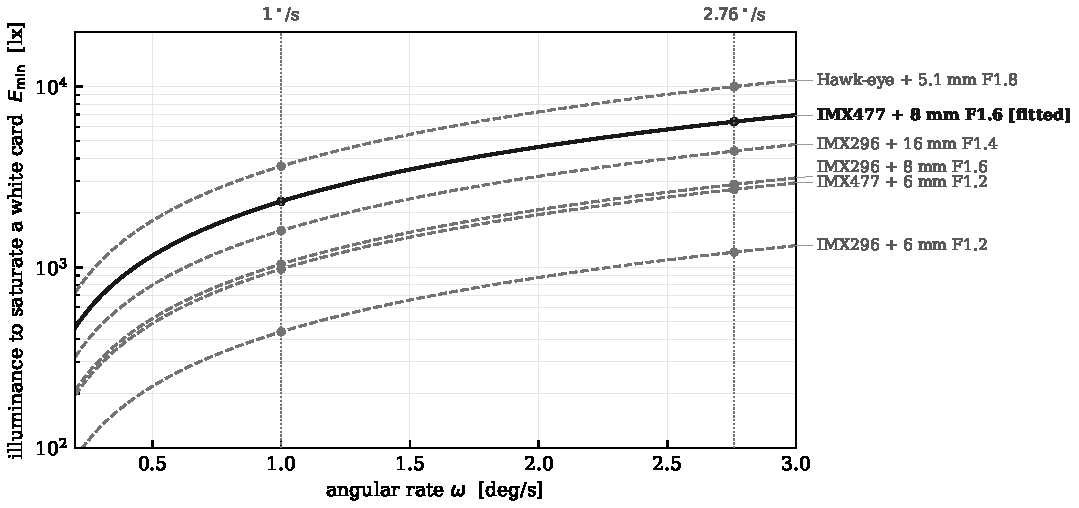
\includegraphics[width=\textwidth]{Images/fig_camera_requirement.pdf}
\caption[Illuminance required as a function of angular rate]{Illuminance required to saturate a white card within the motion-blur ceiling, as a function of angular rate, from Equations \ref{eq:tmax} and \ref{eq:emin}. The requirement is inversely proportional to the available exposure and therefore proportional to $\omega$. Markers show the two rates of Table \ref{tab:light-budget}. Generated by \texttt{make\_figures.py}.}
\label{fig:requirement}
\end{figure}

\subsection{Which configuration sizes the lamp}

The six configurations span 439 to 3622~lx, a range of 3.0 stops, so the lens choice matters as much as the sensor choice. Three readings follow from Table \ref{tab:light-budget}.

\textbf{The Hawk-eye still sets the ceiling}, at 3622~lx, 1.56 times the fitted IMX477 configuration. Its pixel is the smallest of the three sensors, which tightens the exposure ceiling to 9.0~ms, and its fixed F1.8 optic admits $(1.8/1.6)^2 = 1.27$ times less light than the fitted 8~mm lens wide open. If all three cameras are to be exercised in one session, the lamp must be sized for it: roughly \textbf{3600~lx at 1\textdegree/s} and \textbf{10\,000~lx at 2.76\textdegree/s}, measured at the tether position. This is the figure carried into requirement R5 of Chapter \ref{chap:spec}.

\textbf{Dropping the Hawk-eye would lower the requirement to 2317~lx}, the fitted IMX477 configuration, which is 0.6 stops less light.

\textbf{The 8~mm lens costs 1.2 stops relative to the 6~mm} on the same IMX477 sensor, 2317~lx against 978~lx. Both terms push the same way: the longer focal length narrows the IFOV and so shortens the exposure ceiling from 14.8 to 11.1~ms, and F1.6 admits $(1.6/1.2)^2 = 1.78$ times less light than F1.2. What the 8~mm buys in return is sampling, 1.47 pixels across the tether against 1.11 (Table \ref{tab:sampling}), which for a target this close to the sub-pixel limit is the more valuable of the two.

Even the highest requirement, 10\,000~lx, is 3.7 stops below the orbital Sun. The experiment does not need a solar-constant light source; it needs a well-controlled one.

\section{Flicker}
\label{sec:flicker}

\subsection{Mechanism}

A lamp supplied from the alternating-current grid does not emit steadily. Its luminous output rises and falls twice per electrical cycle, so for a supply frequency $f$ the output is periodic with

\begin{equation}
T_{\mathrm{flicker}} = \frac{1}{2f} ,
\label{eq:flicker-period}
\end{equation}

that is 10~ms on a 50~Hz supply and 8.3~ms on a 60~Hz supply \cite{sheinin2018rollingac}. Those periods are the same order of magnitude as every exposure ceiling in Table \ref{tab:light-budget}, which is precisely the regime in which flicker becomes visible in the image.

A rolling-shutter sensor exposes its rows sequentially rather than simultaneously \cite{raspberrypi_camera_docs}. Row $k$ therefore integrates the lamp waveform over a window displaced by $k$ row periods, and when the exposure is short this inter-row delay turns a temporal fluctuation into a spatial pattern across the frame \cite{sheinin2018rollingac}. The same banding mechanism is reported for sources dimmed by pulse-width modulation \cite{zhu2025rifle}. Figure \ref{fig:flicker} computes the result for the IMX477 at the 2.76\textdegree/s exposure ceiling.

\begin{figure}[!ht]
\centering
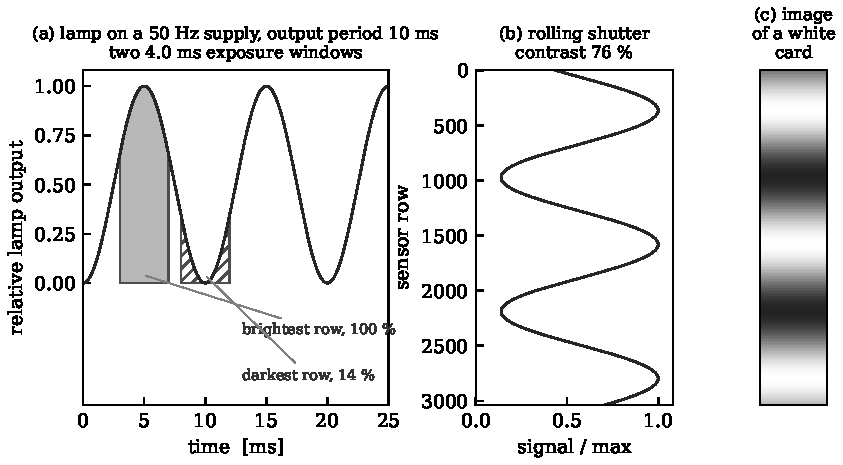
\includegraphics[width=\textwidth]{Images/fig_flicker_banding.pdf}
\caption[Banding produced by an AC-powered lamp on a rolling-shutter sensor]{Flicker banding, computed for a lamp output $L(t) = \sin^{2}(2\pi f t)$ on a 50~Hz supply, an exposure of 4.0~ms, which is the fitted configuration's ceiling at 2.76\textdegree/s, and a 25~ms full-frame readout over 3040 rows, giving a row period of 8.22~\textmu s. (a) The waveform, with the brightest and the darkest 4.0~ms window marked. (b) The signal accumulated by each row. (c) The resulting image of a uniformly lit white card. The 25~ms readout spans 2.5 flicker periods, so 2.5 bands appear. Generated by \texttt{make\_figures.py}.}
\label{fig:flicker}
\end{figure}

\subsection{How bad it gets, and the one exposure that escapes}

Applying the non-uniformity definition of Equation \ref{eq:nu} to the row signals of Figure \ref{fig:flicker}(b) gives a banding contrast that depends strongly on exposure time, as shown in Table \ref{tab:flicker-contrast}. The pattern has a clear structure: when the exposure equals an exact multiple of the flicker period, every row integrates exactly the same amount of light and the banding vanishes, which is the condition Sheinin et al. describe as emulating direct-current illumination \cite{sheinin2018rollingac}. On a 50~Hz supply the computed contrast is exactly zero at 10.0 and 20.0~ms, and rises steeply as the exposure falls below one period: the fitted configuration's 4.0~ms ceiling at 2.76\textdegree/s gives 75.7\%, meaning the darkest band carries about one seventh the signal of the brightest.

\begin{table}[!ht]
\centering
\small
\caption[Banding contrast as a function of exposure time]{Banding contrast across the frame for a 50~Hz supply and a 25~ms readout, from the model of Figure \ref{fig:flicker}. The exposures listed are the ceilings of Table \ref{tab:light-budget} plus the two flicker-free exposures. Computed by \texttt{make\_figures.py}.}
\label{tab:flicker-contrast}
\begin{tabular}{llc}
\toprule
\textbf{Exposure} & \textbf{Where it comes from} & \textbf{Banding contrast} \\
\midrule
3.3 ms  & Hawk-eye ceiling at 2.76\textdegree/s            & 83.0\% \\
\textbf{4.0 ms}  & \textbf{fitted IMX477 ceiling at 2.76\textdegree/s} & \textbf{75.7\%} \\
4.5 ms  & IMX296 + 16 mm ceiling at 2.76\textdegree/s      & 68.5\% \\
5.4 ms  & IMX477 + 6 mm ceiling at 2.76\textdegree/s       & 58.5\% \\
9.0 ms  & Hawk-eye at 1\textdegree/s; IMX296 + 8 mm at 2.76\textdegree/s & 10.9\% \\
10.0 ms & \emph{exactly one flicker period}                & \emph{0.0\%} \\
\textbf{11.1 ms} & \textbf{fitted IMX477 ceiling at 1\textdegree/s}   & \textbf{9.7\%} \\
12.4 ms & IMX296 + 16 mm ceiling at 1\textdegree/s         & 17.6\% \\
14.8 ms & IMX477 + 6 mm ceiling at 1\textdegree/s          & 21.5\% \\
20.0 ms & \emph{exactly two flicker periods}               & \emph{0.0\%} \\
24.7 ms & IMX296 + 8 mm ceiling at 1\textdegree/s          & 12.8\% \\
32.9 ms & IMX296 + 6 mm ceiling at 1\textdegree/s          & 7.6\% \\
\bottomrule
\end{tabular}
\end{table}

Relying on that coincidence is not a viable strategy here, because the exposure time is not free: it is set by Equation \ref{eq:tmax} from the rotation rate under test. The conclusion is that the fixture itself must not flicker.

\subsection{What that requires of the fixture}

For HMI lamps the ballast decides the outcome, and the manufacturer documentation is explicit. ARRI's electronic ballast for the 12/18~kW lamp class, the same class used as the sun simulator at EPOS, lists ``flicker free light'' with a ``typical light ripple max. 3\%'' among its advantages over magnetic ballasts, and offers three modes \cite{arri_eb1218_manual}:

\begin{itemize}
    \item \textbf{50/60 Hz, low noise.} Quieter, but the manual states the light is ``NOT flicker free any more'', with the same camera restrictions as a magnetic ballast.
    \item \textbf{75 Hz, flicker free.} The lamp runs on a 75~Hz square wave and gives constant light, designed for standard film speeds.
    \item \textbf{High speed.} The lamp runs at about 1000~Hz square wave, period 1.00~ms, also flicker free.
\end{itemize}

Given exposures as short as 3.3~ms, the high-speed mode is the appropriate choice, since its 1.00~ms period is short compared with every ceiling in Table \ref{tab:light-budget}. The 75~Hz mode, whose 13.33~ms period exceeds most of those ceilings, is not. For LED fixtures no equivalent statement was found in any reviewed source: the dimming method and pulse-width-modulation frequency must be requested from the manufacturer, and the fixture accepted only after the on-site test.

The global-shutter IMX296 exposes every pixel at once \cite{raspberrypi_camera_docs} and therefore shows no banding, but it is not immune. Its frame brightness still depends on where the exposure window falls within the flicker cycle, as Figure \ref{fig:flicker}(a) shows directly: two windows of equal duration collect 100\% and 14\% of the maximum. On a global-shutter sensor that becomes frame-to-frame brightness variation instead of within-frame banding, which is equally destructive for a stereo pair that must be radiometrically consistent.
